\section{Recurso solar}\label{sec:recurso}

\subsection{Diagramas cilíndricos del sitio}

La posición del Sol se describe con dos ángulos: la altura solar $h$, medida desde el plano horizontal, y el acimut $\alpha$, medido sobre el horizonte. En este trabajo el acimut se mide desde el norte y en sentido horario (\SI{90}{\degree} al este, \SI{180}{\degree} al sur).

Para calcular estos ángulos se trabajó con el tiempo solar $t_s$, que se obtiene a partir de la hora local $t_u$ con
\begin{equation}
t_s = t_u + \frac{L - L_R}{15} + \Delta_{\mathrm{eot}},
\label{eq:ts}
\end{equation}
donde $L=\SI{-83.70}{\degree}$ es la longitud del sitio, $L_R=\SI{-90}{\degree}$ es la longitud de referencia de Costa Rica y $\Delta_{\mathrm{eot}}$ es la ecuación del tiempo, en horas. Con este resultado el mediodía solar ocurre entre las 11:18 y las 11:49, hora local, según la época del año.

El ángulo horario $\omega$, la declinación $\delta$, la altura solar $h$ y el acimut $\alpha_S$ se calcularon con
\begin{align}
\omega &= 15\,(t_s - 12), \label{eq:omega}\\
\delta &= \sin^{-1}\!\big[0.3978\sin\!\big(\bar d - 1.400 \nonumber\\ &\qquad + 0.0355\sin(\bar d - 0.0489)\big)\big], \label{eq:decl}\\
\sin h &= \sin\varphi\,\sin\delta + \cos\varphi\,\cos\delta\,\cos\omega, \label{eq:altura}\\
\sin \alpha_S &= \frac{\cos\delta\,\sin\omega}{\cos h}, \label{eq:acimut}
\end{align}
donde $\varphi=\SI{9.377}{\degree}$ es la latitud y $\bar d = 2\pi d/365.25$ el ángulo diario, en radianes, con $d$ el día del año ($d=1$ el 1 de enero). El acimut de \eqref{eq:acimut} se mide desde el sur; cuando el Sol pasa al norte del cenit se corrigió el cuadrante y el resultado se refirió al norte.

La Fig.~\ref{fig:cilindrico} presenta el diagrama cilíndrico del sitio para el día 21 de cada mes, calculado con estas ecuaciones. La Fig.~\ref{fig:cilindrico_uo} muestra el diagrama obtenido con la herramienta de la Universidad de Oregon para las mismas coordenadas \cite{uoregon}. Las trayectorias y las alturas máximas coinciden con las calculadas; las líneas de hora aparecen desplazadas porque esa herramienta usa la hora estándar local y no la hora solar.

\begin{figure*}[!t]
\centering
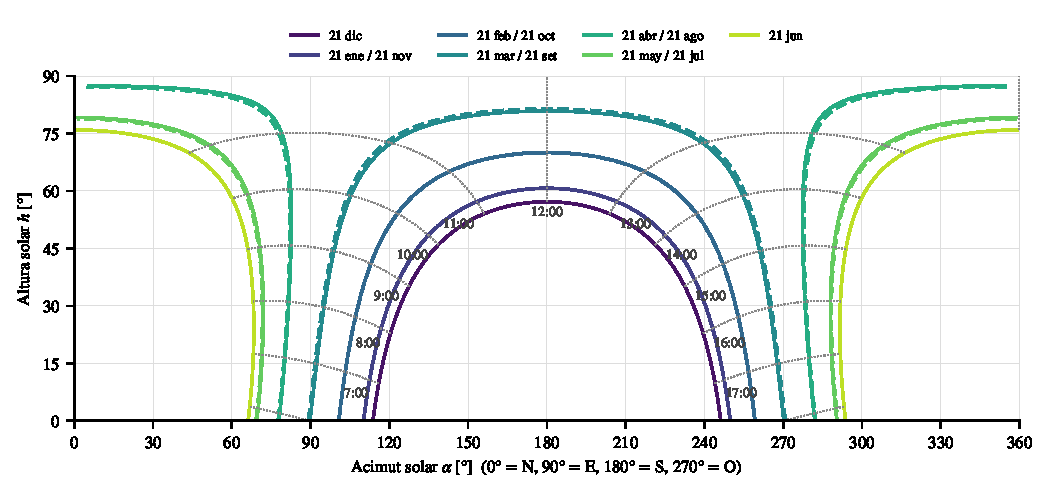
\includegraphics[width=0.85\textwidth]{diagrama_cilindrico.pdf}
\caption{Diagrama cilíndrico del recorrido solar en San Isidro de El General (\SI{9.377}{\degree}\,N), día 21 de cada mes, en tiempo solar. Las líneas punteadas unen puntos de la misma hora.}
\label{fig:cilindrico}
\end{figure*}

\begin{figure*}[!t]
\centering
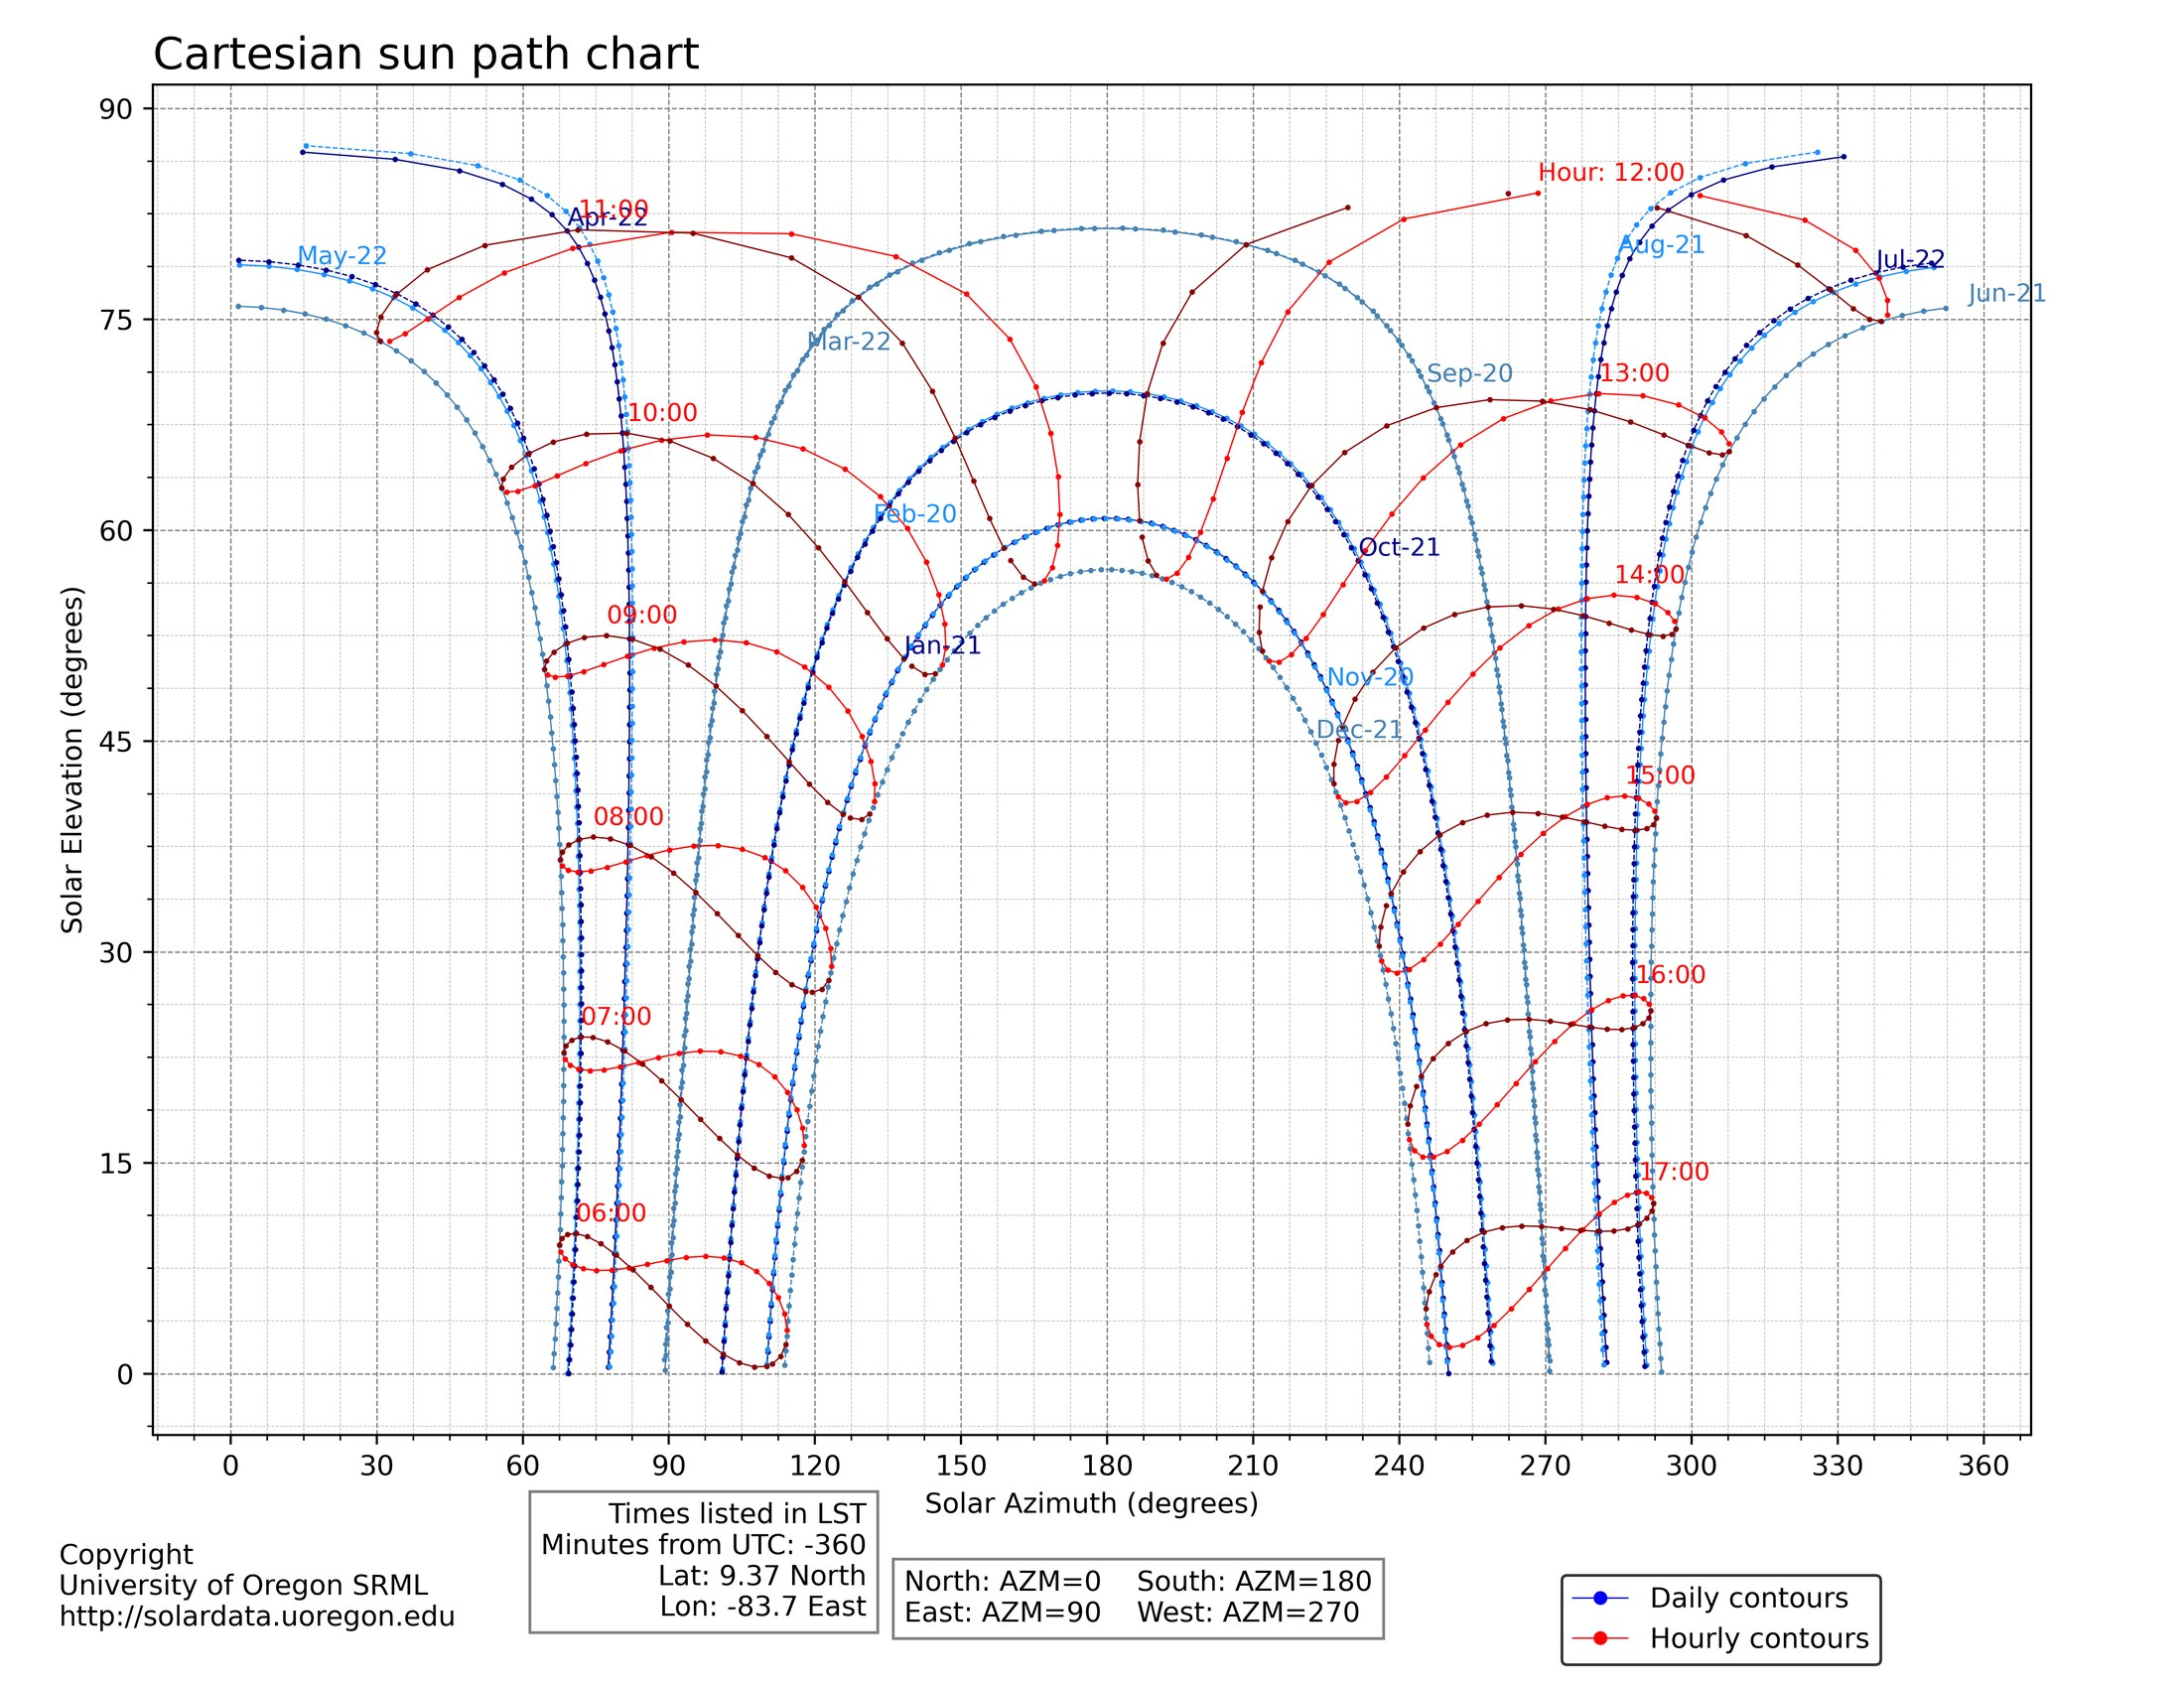
\includegraphics[width=0.72\textwidth]{cilindrico_uoregon.jpg}
\caption{Diagrama cilíndrico del sitio generado con la herramienta de la Universidad de Oregon, en hora estándar local (UTC$-6$) \cite{uoregon}.}
\label{fig:cilindrico_uo}
\end{figure*}

Por la cercanía al ecuador, el Sol pasa muy alto todo el año: al mediodía solar la altura no baja de \SI{57.2}{\degree} (21 de diciembre), y entre mediados de abril y finales de agosto el Sol pasa al norte del cenit. La duración del día también cambia poco, entre \SI{11.45}{h} y \SI{12.55}{h}. Diciembre presenta las menores alturas: a las 10:00 y a las 14:00 (hora solar) del 21 de diciembre la altura es de \SI{46.0}{\degree}, valor que se usa para calcular la separación entre filas de módulos.

\subsection{Componentes de radiación y bases de datos meteorológicas usadas}

La radiación global horizontal (GHI) es la suma de la componente difusa horizontal (DHI) y de la directa proyectada sobre el plano horizontal. Las bases de datos reportan la directa sobre un plano perpendicular a los rayos (DNI), por lo que la GHI no es igual a la suma de la DNI y la DHI, sino que
\begin{equation}
\mathrm{GHI} = \mathrm{DHI} + \mathrm{DNI}\cos\theta_z, \label{eq:ghi}
\end{equation}
donde $\theta_z = \SI{90}{\degree}-h$ es el ángulo cenital. Sobre un plano inclinado se suma una tercera componente, la reflejada por el suelo, que depende del albedo. Con \SI{10}{\degree} de inclinación el módulo casi no ve el suelo: el factor $(1-\cos\beta)/2$ vale 0.008, de modo que con un albedo típico de 0.2 esta componente aporta menos del 0.2\,\% de la GHI.

Se utilizaron dos bases de datos satelitales y, como comprobación, mediciones históricas del Instituto Meteorológico Nacional (IMN):
\begin{itemize}
\item \textbf{\textit{NASA POWER}} \cite{nasa_power}: promedios mensuales de 2001 a 2025 de radiación (estimada desde satélite) y de temperatura. Es la base usada en el diseño.
\item \textbf{\textit{PVGIS} 5.3} \cite{pvgis}: base \textit{PVGIS}-ERA5, promedios de 2005 a 2023 obtenidos de un reanálisis meteorológico. Se usa como comparación.
\item \textbf{IMN} \cite{imn_castro}: radiación global media de la estación Repunta, en Pérez Zeledón (\ang{9;18;}\,N, \ang{83;39;}\,O, \SI{580}{m}), estimada con el brillo solar de 1962 a 1980. Se usa como comprobación.
\end{itemize}
La Tabla~\ref{tab:radiacion} presenta la irradiación diaria promedio de cada mes en \kwhmd; en esta unidad la GHI coincide con las horas solares pico (HSP) sobre el plano horizontal.

\begin{table}[!htb]
\caption{Irradiación diaria promedio mensual [\kwhmd]}
\label{tab:radiacion}
\centering
\small
\setlength{\tabcolsep}{4pt}
\begin{tabular}{l S[table-format=1.2] S[table-format=1.2] S[table-format=1.2] S[table-format=1.2] S[table-format=-2.1]}
\toprule
 & \multicolumn{3}{c}{\textit{NASA POWER}} & {\textit{PVGIS}} & {Dif.} \\
\cmidrule(lr){2-4}
{Mes} & {GHI} & {DNI} & {DHI} & {GHI} & {[\%]} \\
\midrule
Ene & 4.56 & 4.40 & 1.67 & 5.22 & 14.6 \\
Feb & 5.10 & 4.63 & 1.83 & 5.85 & 14.9 \\
Mar & 5.30 & 4.19 & 2.04 & 5.99 & 13.1 \\
Abr & 4.82 & 2.79 & 2.29 & 5.36 & 11.2 \\
May & 4.35 & 2.00 & 2.32 & 4.31 & -0.9 \\
Jun & 4.30 & 1.74 & 2.44 & 4.09 & -5.0 \\
Jul & 4.17 & 1.67 & 2.38 & 4.15 & -0.5 \\
Ago & 4.30 & 1.79 & 2.39 & 4.18 & -2.8 \\
Set & 4.47 & 2.16 & 2.35 & 4.14 & -7.4 \\
Oct & 4.03 & 1.95 & 2.18 & 3.69 & -8.3 \\
Nov & 3.68 & 2.30 & 1.87 & 3.70 & 0.7 \\
Dic & 4.07 & 3.66 & 1.67 & 4.57 & 12.1 \\
\midrule
Prom. & 4.42 & 2.76 & 2.12 & 4.60 & 3.9 \\
\bottomrule
\end{tabular}
\\[2pt]
{\footnotesize Dif.: diferencia de la GHI de \textit{PVGIS} respecto a \textit{NASA POWER}.}
\end{table}

Según \textit{NASA POWER}, la DNI es mayor de diciembre a marzo y la GHI de enero a abril, mientras que de mayo a noviembre la componente difusa supera el 50\,\% de la global (Fig.~\ref{fig:radiacion}). Los valores anuales son de \SI{1615}{kWh/m^2} con \textit{NASA POWER} y \SI{1678}{kWh/m^2} con \textit{PVGIS}, una diferencia de 3.9\,\%. La diferencia se concentra en la época seca, cuando \textit{PVGIS} da entre 11 y 15\,\% más, posiblemente porque ambas bases estiman la nubosidad de forma distinta. La estación Repunta del IMN tiene un promedio de \SI{16}{MJ/m^2} por día, es decir, 4.4~\kwhmd \cite{imn_castro}, prácticamente igual al de \textit{NASA POWER} (4.42). Por eso el diseño se basa en \textit{NASA POWER}: coincide con la estación del IMN, cubre un período más largo y, al dar el valor más bajo, evita sobrestimar la generación.

\begin{figure}[!htb]
\centering
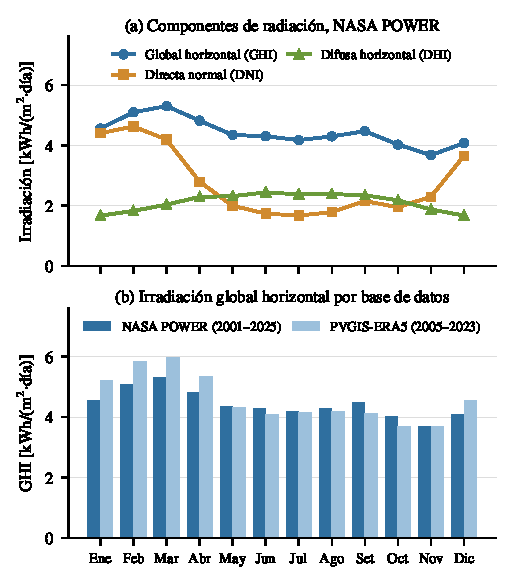
\includegraphics[width=\anchofig]{radiacion_componentes.pdf}
\caption{(a) Componentes de radiación mensuales según \textit{NASA POWER}. (b) Comparación de la irradiación global horizontal entre \textit{NASA POWER} y \textit{PVGIS}.}
\label{fig:radiacion}
\end{figure}

Los promedios mensuales ocultan la variación que existe de un día a otro. Para observarla se consultaron en \textit{NASA POWER} las series diarias de 2025 de las tres componentes en cielo real, es decir, incluyendo el efecto de las nubes \cite{nasa_power_diario}. En la Fig.~\ref{fig:diaria} se observa que un día cualquiera puede alejarse bastante del promedio del mes. La directa normal es la más sensible a las nubes: es alta de diciembre a marzo y cae de forma marcada de mayo a noviembre, mientras que la difusa es más estable y gana peso en la época lluviosa, cuando sostiene la producción en días nublados. El promedio de 2025 fue de 4.31~\kwhmd, un 2.5\,\% menor que el promedio de largo plazo usado para el diseño, lo que muestra que la producción de un año particular puede variar algunos puntos respecto a la estimación.

\begin{figure}[!htb]
\centering
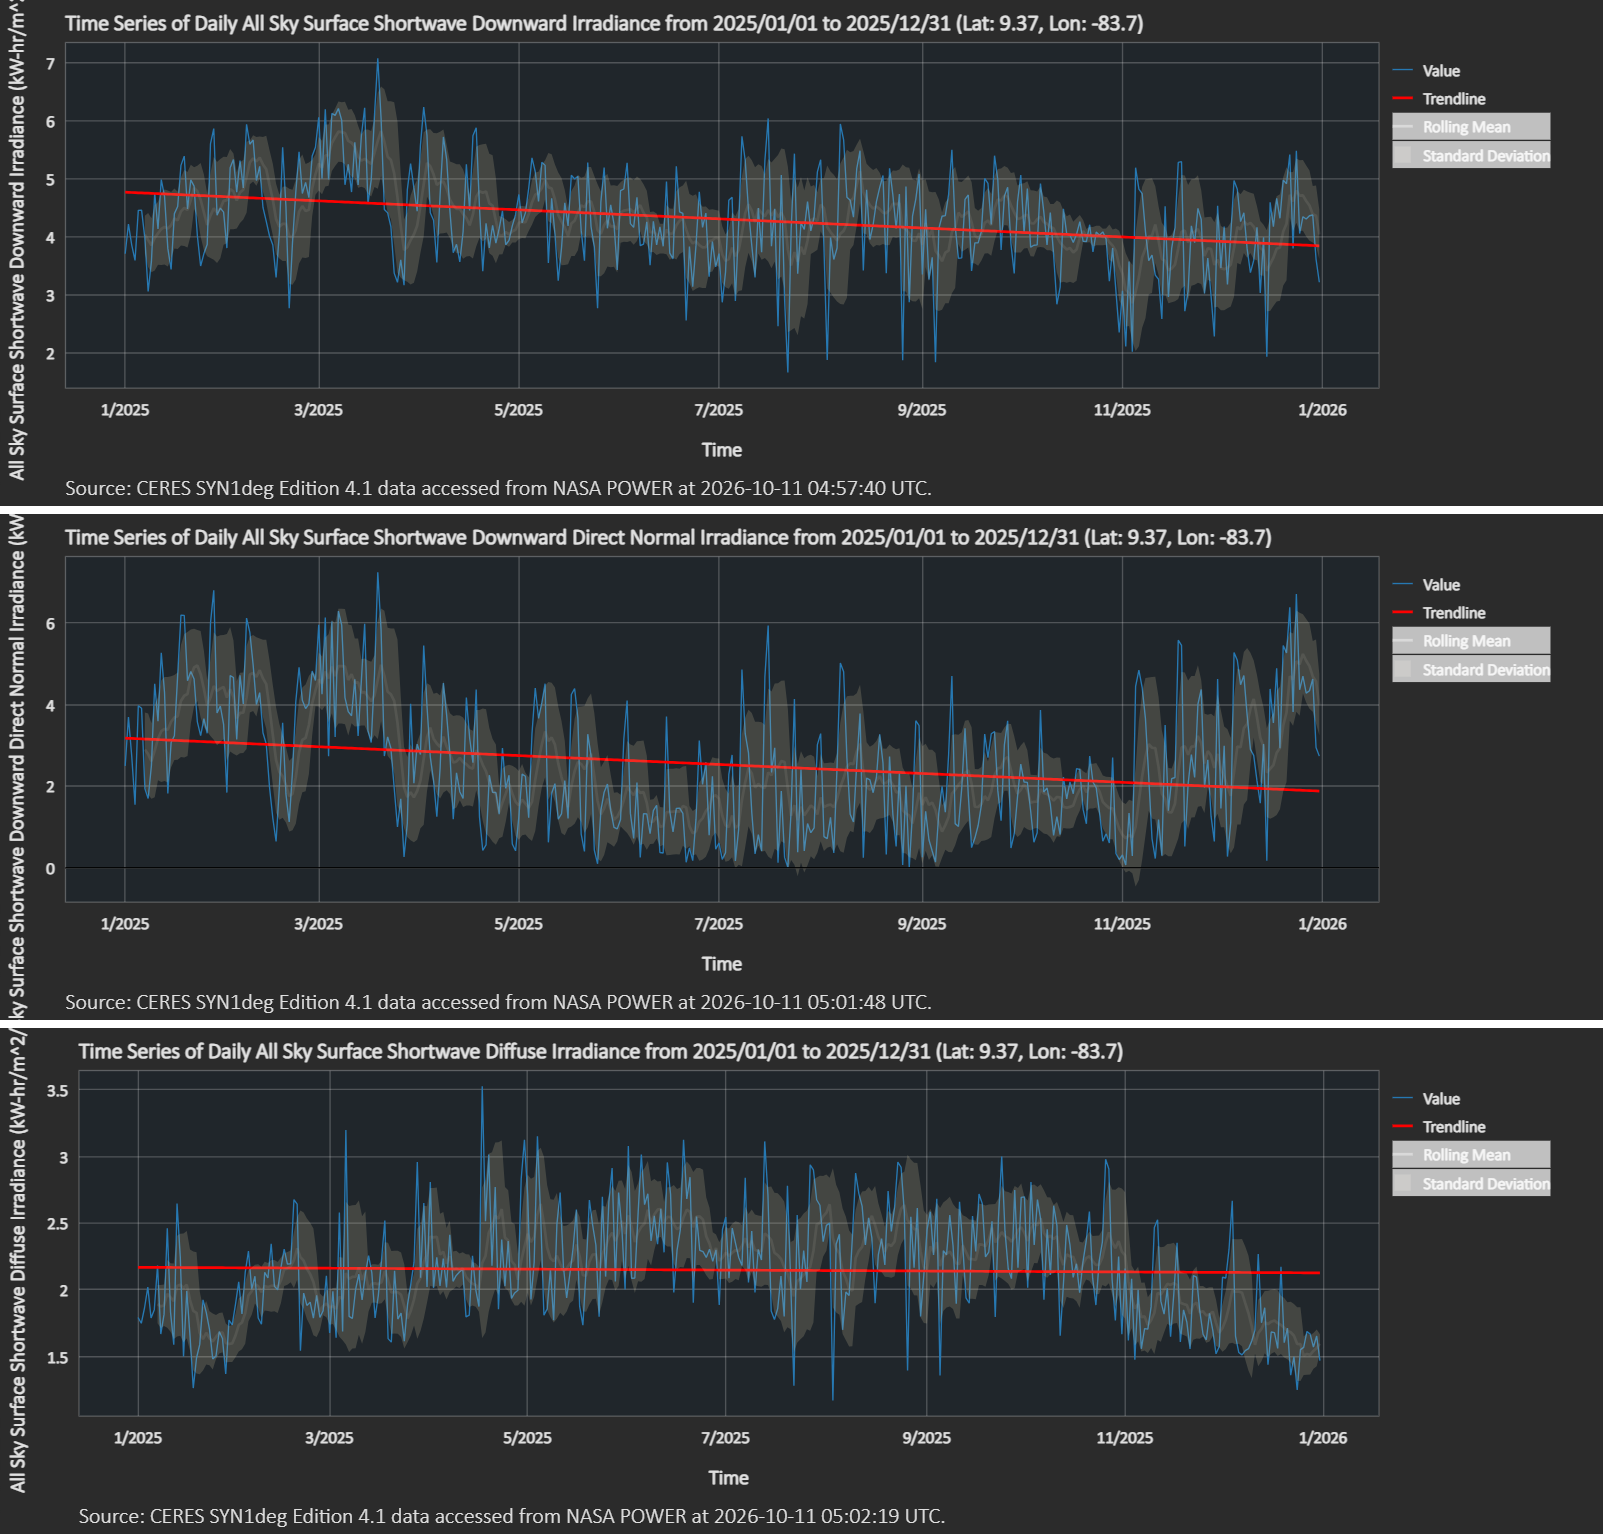
\includegraphics[width=\anchofig,height=0.4\textheight,keepaspectratio]{irradiacion_diaria_2025.png}
\caption{Irradiación diaria en 2025 según \textit{NASA POWER}: (a) global horizontal, (b) directa normal y (c) difusa horizontal, en kWh/(m\textsuperscript{2}$\cdot$día). La línea roja es la tendencia lineal de cada serie \cite{nasa_power_diario}.}
\label{fig:diaria}
\end{figure}

\subsection{Cálculo del ángulo óptimo y comparación con el ángulo disponible}

La radiación sobre un plano inclinado se estimó con los factores de corrección $K$ para una latitud de \SI{10}{\degree}, la más cercana a la del sitio \cite{factores_k}:
\begin{equation}
H_{\beta} = K_{\beta}\,H_{h},
\label{eq:k}
\end{equation}
donde $H_h$ es la irradiación global horizontal y $K_\beta$ el factor para una inclinación $\beta$ hacia el sur. La Tabla~\ref{tab:inclinacion} y la Fig.~\ref{fig:inclinacion} presentan la irradiación anual para las inclinaciones evaluadas.

\begin{table}[!htb]
\caption{Irradiación anual sobre el plano inclinado (orientación sur)}
\label{tab:inclinacion}
\centering
\small
\begin{tabular}{S[table-format=2.0] S[table-format=4.0] S[table-format=-2.1] S[table-format=4.0]}
\toprule
{$\beta$ [°]} & {NASA [kWh/m\textsuperscript{2}]} & {Var. [\%]} & {\textit{PVGIS} [kWh/m\textsuperscript{2}]} \\
\midrule
0  & 1615 & 0.0  & 1678 \\
5  & 1628 & 0.8  & 1692 \\
10 & 1625 & 0.6  & 1691 \\
15 & 1616 & 0.0  & 1682 \\
20 & 1594 & -1.3 & 1661 \\
25 & 1562 & -3.3 & 1629 \\
30 & 1523 & -5.7 & 1589 \\
\bottomrule
\end{tabular}
\\[2pt]
{\footnotesize Var.: variación respecto al plano horizontal con datos de \textit{NASA POWER}.}
\end{table}

\begin{figure}[!htb]
\centering
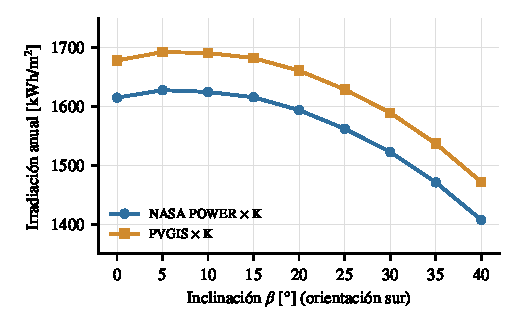
\includegraphics[width=\anchofig]{inclinacion_anual.pdf}
\caption{Irradiación anual en función de la inclinación, con los factores $K$ aplicados a cada base de datos.}
\label{fig:inclinacion}
\end{figure}

Entre los ángulos evaluados, la mayor irradiación anual se obtiene con \SI{5}{\degree}, con una ganancia de 0.8\,\% frente al plano horizontal, y con \SI{10}{\degree} es solo 0.2\,\% menor. Inclinar los módulos favorece los meses de setiembre a marzo, cuando el Sol pasa por el sur, pero reduce la radiación de abril a agosto, cuando pasa por el norte. Con los datos de \textit{PVGIS} el resultado es el mismo: el máximo también se obtiene con \SI{5}{\degree} (Tabla~\ref{tab:inclinacion}).

Como el techo es prácticamente plano, la inclinación la define la estructura. Se eligieron \SI{10}{\degree} hacia el sur en lugar del óptimo de \SI{5}{\degree}. El manual de instalación del módulo pide escoger una inclinación que evite que se acumulen agua y polvo sobre los módulos, e indica que con una inclinación suficiente la lluvia ayuda a limpiar su superficie \cite{aiko_manual}; por eso se prefirió no bajar hasta \SI{5}{\degree}. Este cambio casi no afecta la energía, porque se pierden solo \SI{3}{kWh/m^2} al año (0.2\,\%), y tampoco ocupa más techo, porque la separación adoptada entre filas, de \SI{2.5}{m}, supera la distancia mínima con cualquiera de los dos ángulos (\SI{2.03}{m} con \SI{10}{\degree} y \SI{1.90}{m} con \SI{5}{\degree}; Sección~\ref{sec:instalacion}). Con esta inclinación la irradiación de diseño es de \SI{1625}{kWh/m^2} por año, en promedio \SI{4.45}{HSP}.
